\documentclass[xcolor=dvipsnames]{beamer}
\usepackage[utf8]{inputenc}
\usepackage[IL2]{fontenc}
\usepackage[czech]{babel}
\usepackage{float}
\usepackage{listings}
\usepackage{amssymb}
\usepackage{amsmath}
\usepackage{mathtools}
\usepackage{url}
\usepackage{graphicx}
\usepackage{subfigure}
%\useoutertheme[subsection=false]{smoothbars}
\usetheme{Madrid}
\usecolortheme[named=OliveGreen]{structure}
%\usecolortheme[named=OliveGreen]{structure} 
%\usetheme[height=7mm]{Rochester} 
%\setbeamertemplate{items}[ball] 
%\setbeamertemplate{blocks}[rounded][shadow=true] 
%\useoutertheme{umbcfootline}
\beamertemplatenavigationsymbolsempty 
\title{Kolektivní investování}
\author{Marek Bryša, Jan Kovář}
\institute
{
Masarykova Univerzita\\
Přírodovědecká fakulta
}
\date{\today}

\begin{document}
  \frame{\titlepage}
\begin{frame}
\section*{Úvod}
  \frametitle{Úvod}
  \begin{itemize} 
    \item Kolektivní investování je definováno v zákoně č. 189/2004 Sb., o kolektivním investování .
\begin{block}{Definice kolektivního investování}
Kolektivní investování je podnikání, jehož předmětem je
shromažďování peněžních prostředků upisováním akcií investičního fondu nebo vydáváním
podílových listů podílového fondu, investování na principu rozložení rizika a další
obhospodařování tohoto majetku.
  \end{block}
  \end{itemize} 

\end{frame}


%\begin{frame}

%\section{Subjekty kolektivního investování}
%\frametitle{Obsah}
%\tableofcontents[currentsection]

%\end{frame}


\begin{frame}
\frametitle{Subjekty kolektivního investování} 
\begin{itemize}
  \item Investiční společnost
  \item Investiční fond
  \item Podílový fond
\end{itemize}
\end{frame}

\begin{frame}
\frametitle{Investiční společnost}
\begin{itemize} 
  \item Právnická osoba,
  \item jejímž předmětem podnikání je kolektivní investování
  \item Může
    \begin{itemize} 
      \item zakládat podílové fondy a spravovat majetek do nich vložený
      \item obhospodařovat majetek investičních fondů na základě smlouvy o~obhospodařování
    \end{itemize}
  \item Ke své činnosti musí investiční společnost získat povolení České národní banky
\end{itemize} 
\end{frame}

\begin{frame}
\frametitle{Investiční fond}
\begin{itemize} 
\item Právnická osoba (akciová společnost), 
\item jejímž předmětem podnikání je kolektivní investování 
\item a která má povolení ČNB k~činnosti investičního fondu
\item Zakládá se na dobu určitou (max. na 10~let)
\item Obchodní firma investičního fondu musí obsahovat označení \emph{uzavřený investiční fond}
\item Investiční fond může vydávat pouze akcie stejné jmenovité hodnoty
\item Na základě smlouvy o~obhospodařování majetku může investiční fond svěřit obhospodařování svého majetku investiční společnosti
\end{itemize} 
\end{frame}


\begin{frame}
\frametitle{Podílový fond}
\begin{itemize} 
\item Nemá právní subjektivitu
\item Je zakládán investiční společností
\item na základě povolení České národní banky
\item Investiční společnost shromažďuje prostředky do podílového fondu vydáváním podílových listů
\item Podílový list je cenný papír, který představuje podíl na majetku podílového fondu
\item Podílový fond je souborem majetku, který náleží všem vlastníkům podílových listů, tzv. podílníkům, a to dle poměru držených podílových listů  
\end{itemize} 
\end{frame}


\begin{frame}
\frametitle{Podílové fondy - dělení}
\begin{itemize}
  \item Otevřený podílový fond
    \begin{itemize}
      \item má povinnost zpětného odkupu podílových listů
      \item nemá předem omezen počet emitovaných podílových listů
      \item nemá omezen počet podílníků
     \end{itemize}
  \item Uzavřený podílový fond
    \begin{itemize}
     \item má již při svém vzniku stanoven počet podílových listů, které může emitovat
     \item zakládán na dobu určitou
     \item po této době vstupuje do likvidace, anebo se změní na otevřený fond
    \end{itemize}
\end{itemize}  
\end{frame}


\begin{frame}
\frametitle{Fondy kolektivního investování}
\begin{figure}[htb]
\centering
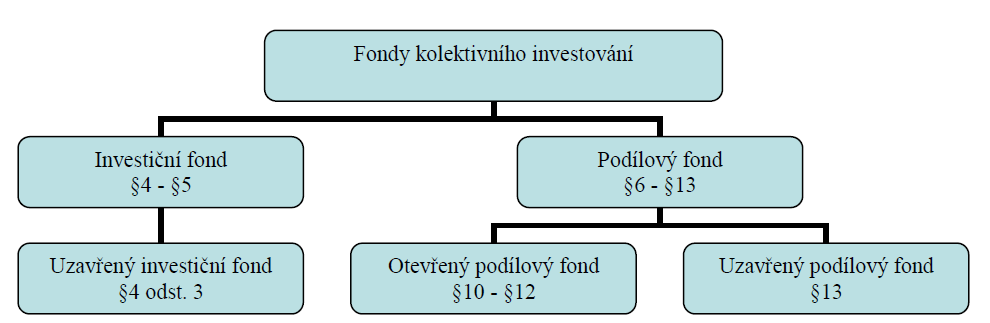
\includegraphics[width=\textwidth]{deleni.png}
\caption{Členění fondů kolektivního investování dle zákona č. 189/2004 Sb., o kolektivním investování, zdroj: \cite{dp}}
\end{figure}
\end{frame}

  

%\begin{frame}
%\section{Výhody a nevýhody kolektivního investování}
%
%\frametitle{Obsah}
%\tableofcontents[currentsection]
%
%\end{frame}




 
\begin{frame}
  \frametitle{Výhody kolektivního investování} 
    \begin{itemize} 
\item Diverzifikace rizika
\item Snížení transakčních nákladů 
\item Likvidita vložených prostředků
\item Profesionální správa majetku
\item Možnost investovat do titulů, ke kterým by se drobný investor samostatně nedostal
\item Dohled regulátorů
\end{itemize} 
\end{frame}




\begin{frame}
\frametitle{Nevýhody kolektivního investování} 
\begin{itemize} 
\item Správní poplatky
\item Omezení investiční volnosti
\item Konflikt zájmu mezi investory a správci portfolia
\item Často podprůměrná výkonnost fondů
\item Riziko investování
\end{itemize} 
\end{frame}

	\section{Vybrané fondy v České republice}
		\begin{frame}{AXA investiční společnost, a.s.}
			\begin{center}
				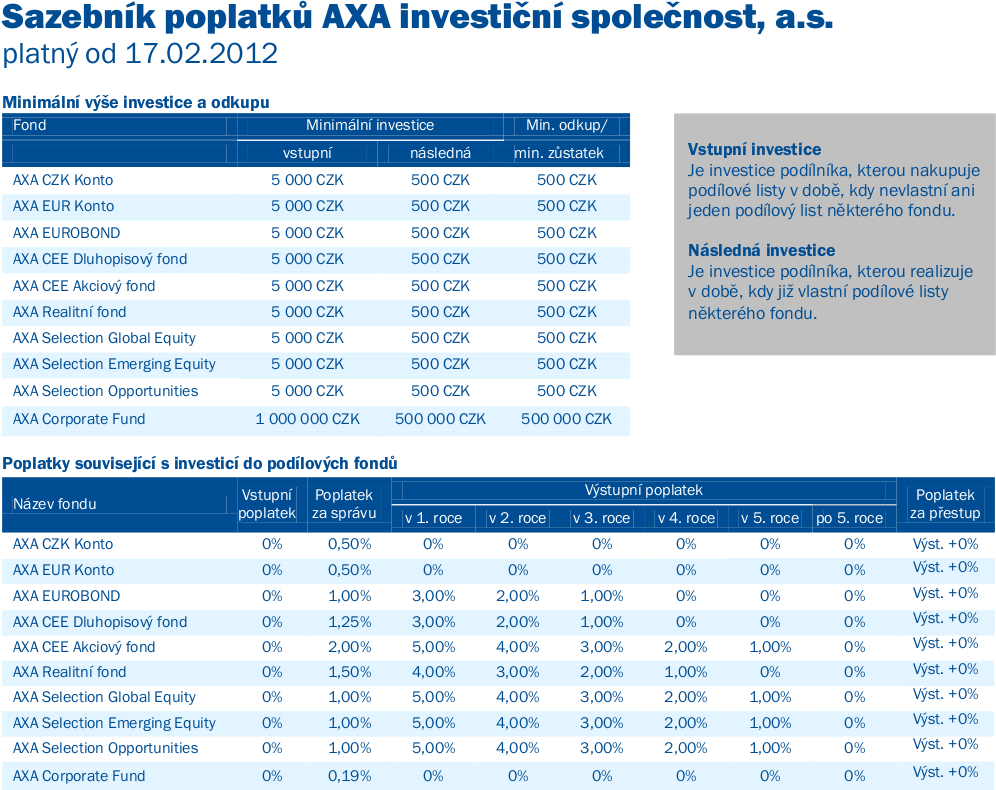
\includegraphics[width=0.8\textwidth]{axa_popl.png}			
			\end{center}
		\end{frame}
		\subsubsection{AXA CZK Konto}
			\begin{frame}{AXA CZK Konto}
				\begin{quote}
				Cílem investiční strategie je poskytnout podílníkům růst hodnoty jejich investice za podmínky, že celkový rizikový profil fondu minimalizuje možnost ztráty v horizontu 6 měsíců. Cíle je dosahováno investicemi do široce diverzifikovaného portfolia cenných papírů s fixním nebo variabilním úrokovým výnosem a aktivním řízením úrokového rizika.\footnote{\url{http://www.axa.cz/lide/podilove-fondy/czk-konto/popis}}
				\end{quote}
			\end{frame}
			\begin{frame}{AXA CZK Konto}
				\begin{center}
					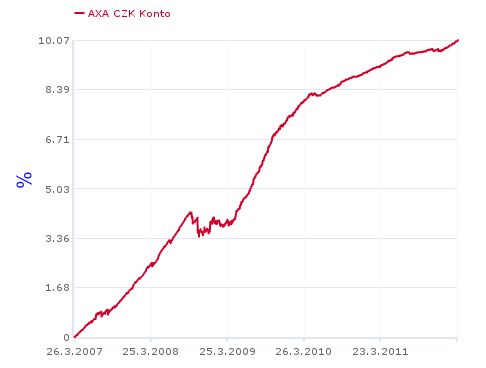
\includegraphics[width=0.7\textwidth]{axa_czk_konto.png}
				\end{center}							
				Výkon za 5 let 10.07\%, což je 1.93\% ročně, za poslední rok 0.8\%.
			\end{frame}
			\begin{frame}{AXA CEE Dluhopisový fond}
			\begin{quote}
				Fond investuje do dluhopisů emitentů všech kategorií:
				\begin{itemize}
			    \item dluhopisů nadnárodních institucí
			    \item státních dluhopisů
			    \item bankovních dluhopisů
			    \item dluhopisů obchodních společností
			    \item komunálních dluhopisů emitovaných v krajinách střední a východní Evropy\footnote{\url{http://www.axa.cz/lide/podilove-fondy/cee-dluhopisovy/popis}}	
    	  \end{itemize}
		  \end{quote}
		  Doporučeným investičním horizontem jsou minimálně 3 roky. Fond je určen pro střednědobé investice s mírou rizika i výnosem o něco výššími než u fondu peněžního trhu.
			\end{frame}
			\begin{frame}{AXA CEE Dluhopisový fond}
				\begin{center}
					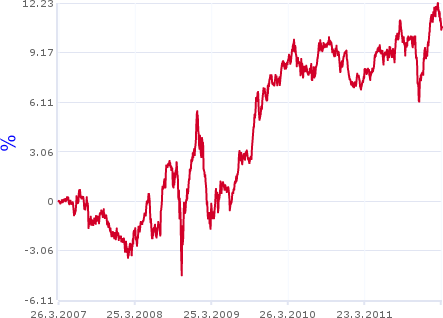
\includegraphics[width=0.7\textwidth]{axa_cee_dluh.png}
				\end{center}							
				Výkon za 5 let 10.73\%, což je 2.05\% ročně.\\
				Monhem vyšší volatilita.
			\end{frame}
			\begin{frame}{AXA CEE Akciový fond}
				\begin{quote}
				Cílem fondu je dosahovat co nejvyššího dlouhodobého zhodnocení investic. Majetek fondu je tvořený především akciemi společností, které jsou lídry ve svém odvětví v regionu střední a východní Evropy. Největší podíl na portfoliu mají české, polské a maďarské společnosti. Odvětvová struktura portfolia není omezená, významně se na ní ale podílí energetický, telekomunikační a finanční sektor. Investice jsou směřované také do odvětví farmacie či strojírenství.\footnote{\url{http://www.axa.cz/lide/podilove-fondy/cee-akciovy/popis}}
			\end{quote}
			Doporučeným investičním horizontem je minimálně 5 let. Fond pro ivestora slibuje vyskoké zhodnocení v dlouhém období, ale za cenu vysoké střednědobé volatility.
			\end{frame}
			\begin{frame}{AXA CEE Akciový fond}
				\begin{center}
					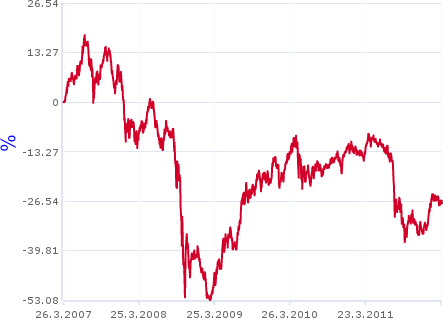
\includegraphics[width=0.7\textwidth]{axa_cee_akc.png}
				\end{center}							
				Za 5 let fond ztratil 27.11\% hodnoty, v době finanční krize dokonce 52.3\%.
			\end{frame}
	\subsection{Pioneer Asset Management, a.s. -- Rentier Invest}
	\begin{frame}{Pioneer Asset Management, a.s. -- Rentier Invest}
		Program tvoří 7 na sebe navazujících linií s postupně se snižující rizikovostí a výnosem.
		\begin{center}
			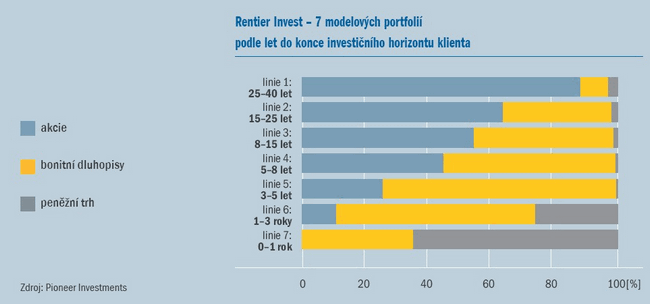
\includegraphics[width=0.9\textwidth]{graf_alokace_linii.png}
		\end{center}
	\end{frame}
	\begin{frame}{Rentier Invest}
		Minimálně je možno investovat poprvé 30 000 Kč, následně 10 000 Kč nebo pravidelně 1 000 Kč.
		\begin{center}
			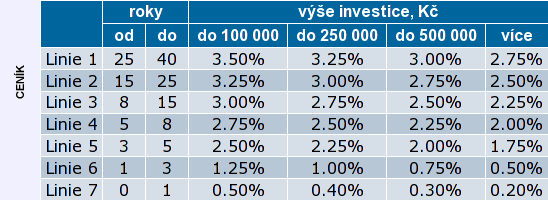
\includegraphics[width=0.9\textwidth]{ri_cost.png}
		\end{center}
	\end{frame}
		\begin{frame}{Rentier Invest}
		\begin{center}
			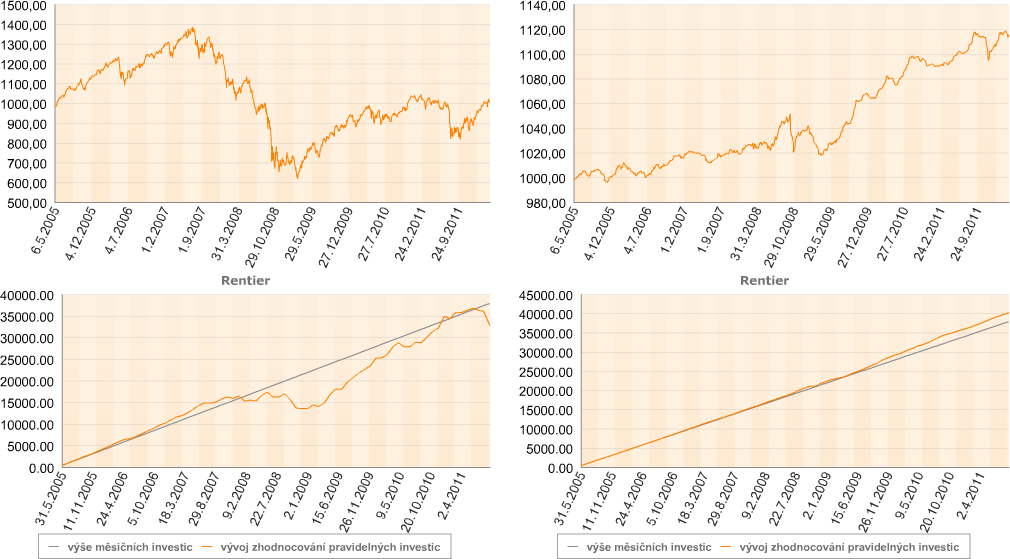
\includegraphics[width=1.0\textwidth]{ri_graf.png}
		\end{center}
		Linie 1 dosáhla za posledních 5 let ztráty 22.08\%, linie 7 zisku 9.27\%.
	\end{frame}
\end{document}